\chapter{Results}

\section{Steering Clear Reproduction}

\begin{figure}
    \centering
    \captionsetup{width=\textwidth}
    \includegraphics[width=\textwidth]{figures/steering_clear.png}
    \caption{
        Reproduction of Figure 1 (top-left) in \citet{steering-clear}.
        Instead of overlaying all the data in a single plot the for methods are separated.
        ACE \citep{ace} is introduced and MiMiC \citep{mimic} is removed.
        Though the metric is different, focusing on the steered attribute rather than all attributes, the same trends are presents.
        The model accuracy is changed to reflect the accuracy of the model without steering rather than the model accuracy on the target input.
    }
    \label{fig:gpt-pp-sae}
\end{figure}

\section{Prompt Pairs}

\begin{figure}
    \centering
    \captionsetup{width=\textwidth}
    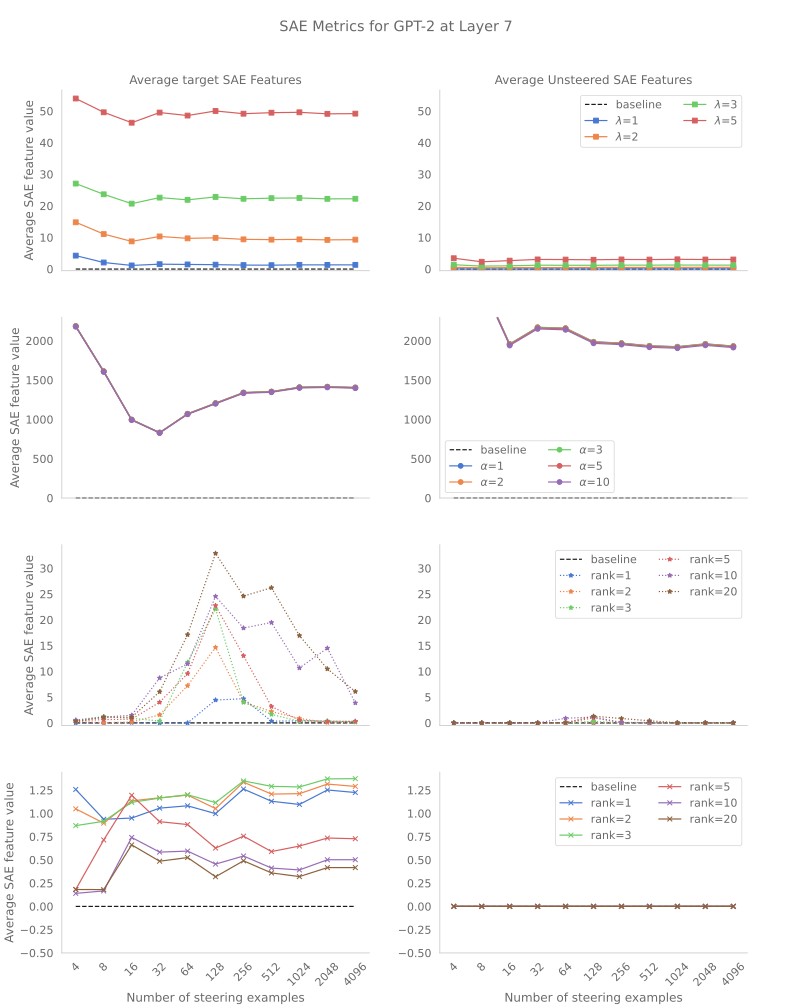
\includegraphics[width=\textwidth]{figures/gpt2_7_sae.png}
    \caption{
        The average activation of SAE features for the set of target SAE features and unsteered SAE features.
        From top to bottom the rows represent CAA \citep{caa}, ACE \citep{ace}, LoReFT \citep{reft} and LoReST \citep{steering-clear}.
        The same range of examples is used across all adaptors.
        The exact SAE feature values are only important in the unsteered case, where they should be 0, or as a comparison within the model parameters.
    \Sref{sec:prompt-pairs} describes how these metrics are calculated.}
    \label{fig:gpt-pp-sae}
\end{figure}

\begin{figure}
    \centering
    \captionsetup{width=.9\textwidth}
    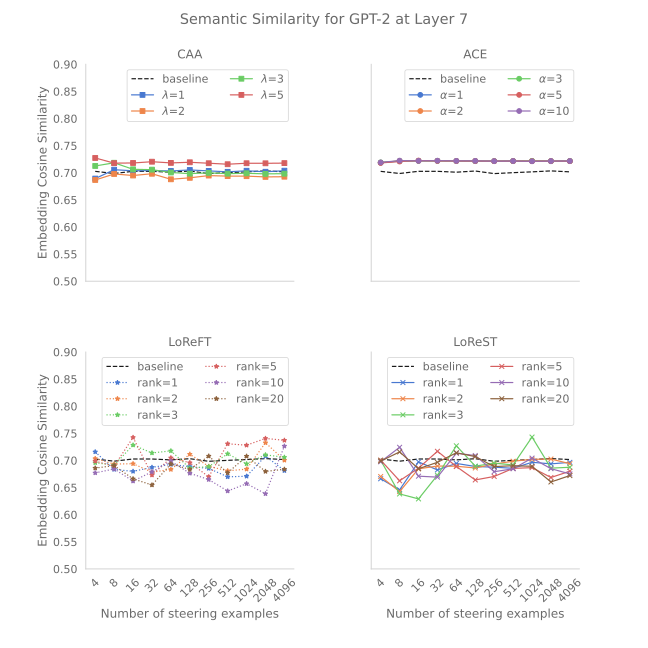
\includegraphics[width=\textwidth]{figures/gpt2_7_similarity.png}
    \caption{
        The cosine similarity of distilbert \citep{distilbert} word embeddings for the generated token.
        The number of steering examples is the same as \Fref{fig:gpt-pp-sae} and the cosine similarity is shared across charts.
        Note that the y axis has been cropped to highlight the difference between models though the change is slight.
    }
    \label{fig:gpt-pp-sim}
\end{figure}

